\documentclass[a4paper, titlepage]{article}
\usepackage[utf8]{inputenc}
\usepackage[T1]{fontenc}
\usepackage[magyar]{babel}
\usepackage{graphicx}
\usepackage{geometry}
\geometry{margin=1.2in}
\begin{document}
\begin{titlepage}
	\title{\textbf{Folytonos közegek mechanikája}\\
	Tételkidolgozás\\
	9. tétel\\
	\textit{Súrlódó folyadék, a feszültségtenzor alakja, áramlás csőben}}
	\author{Készítette Pesznyák Dávid\\
	Dr. Groma István előadásai alapján (2018)}
	\date{}
\end{titlepage}
\maketitle
\newpage
\subsection*{A súrlódó folyadékok modelljének alapja}
A folyadékok súrlódásával először Sir Isaac Newton foglalkozott még a 17. században. Kísérletében egy vízzel teli medencébe helyezett egy fából készült testet, majd arra állandó nagyságú, a vízfelszínnel párhuzamos erőt fejtett ki. Arra lett figyelmes, hogy eddigi megfigyeléseivel ellentétben a test egyenletesen gyorsuló mozgás helyett állandó sebességgel kezdett  mozogni.\\\\
\begin{figure}[h]
\begin{center}
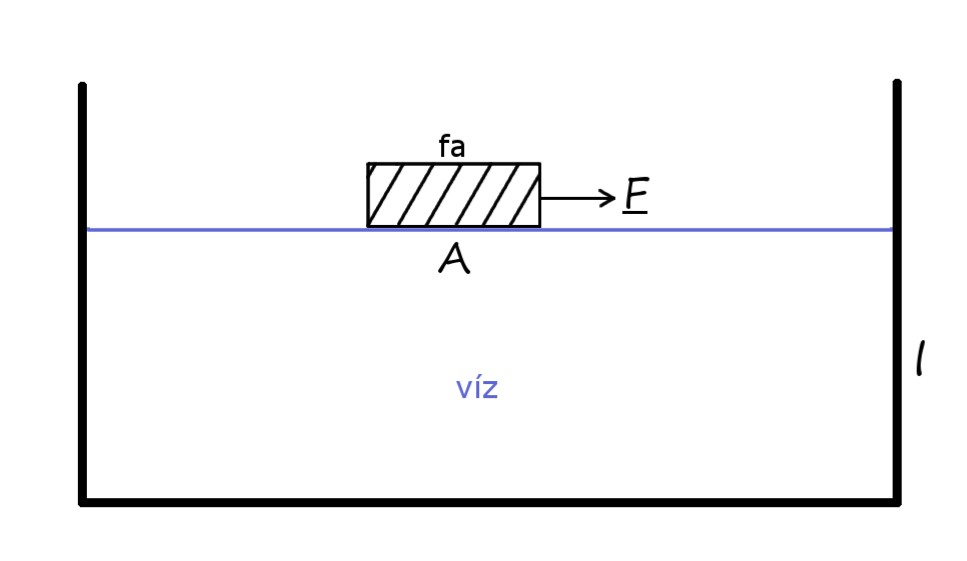
\includegraphics[scale=0.3]{Newton.JPG}
\end{center}
\end{figure}
\\\\A megfigyelések alapján a testet egyenletes mozgásra kényszerítő erőt a következő formában írhatjuk fel:
\begin{equation}
F=\eta\; \frac{v A}{l},
\end{equation}
ahol $v$ a test sebessége, $A$ a test vízzel érintkező felületének felszíne, $l$ a medence mélysége és $\eta$ a viszkozitási együttható.\\\\
A mozgás során a vízzel párhuzamosan nyírás megy végbe, azonban a nyírófeszültség jelen esetben nem a már tanult $\tau=\frac{F}{A}=\eta \frac{v}{l}$ összefüggés fogja megadni, hanem a következő képlet lesz érvényes:
\begin{equation}
\tau=\eta\; \frac{dv_x}{dz},
\end{equation}
Ezt nevezzük a \textit{Newton-féle viszkozitási törvénynek}.
\subsection*{A feszültségtenzor alakja}
Mivel tudjuk, hogy a deformációs tenzor ($\hat{\varepsilon}$) komponensei:
$$\varepsilon_{ij}=\frac{1}{2}\;\bigg(\frac{\partial u_i}{\partial r_j}+\frac{\partial u_j}{\partial r_i}\bigg),$$
és ezek alapján a deriváltja ($\dot{\hat{\varepsilon}}$):
$$\dot{\varepsilon}_{ij}=\frac{1}{2}\;\bigg(\frac{\partial v_i}{\partial r_j}+\frac{\partial v_j}{\partial r_i}\bigg)$$
Észrevehetjük, hogy $\frac{dv_x}{dz}$ éppen $\dot{\varepsilon}_{12}$-vel egyenlő, így arra a következtetsére juthatunk, hogy a szilárd anyagokkal ellentétben a folyadékoknál a feszültségtenzor ($\hat{\sigma}$) nem a deformációs tenzortól, hanem annak deriváltjától függ. Ez abban is megnyilvánul, hogy a kialakuló sebességtér helyfüggő lesz.\\\\
Ezek alapján felírható általánosan a feszültségtenzor:
\begin{equation}
\label{equ:sigma}
\hat{\sigma}=-p\;\hat{I}\; +\; \hat{\sigma}'(\dot{\hat{\varepsilon}}),
\end{equation}
ahol $p$ skalár szorozva az "egységtenzorral" a nyomásból adódó feszültséget jelenti, a $\hat{\sigma}'$-s tagot pedig ezek után részletezzük.
\subsection*{Lineáris közelítés}
A szilárd anyagok esetében feltehettük, hogy a $\hat{\sigma}(\hat{\varepsilon})$ összefüggés lineáris, de ez a feltevés már nem teljesül minden folyadékra. Azokat a folyadékokat, amelyek esetében igaz ez a lineáris kapcsolat Newton-i folyadékoknak nevezzük (tehát $\hat{\sigma}'(\dot{\hat{\varepsilon}})$ lineáris). Továbbá, mivel a folyadékokban nincsenek kitüntetett irányok, izotrópnak tekinthetők, így a \textit{Hooke-törvény} a következő alakban írható fel rájuk a szilárd testekre felírt kifejezés analógiájából:
\begin{equation}
\label{equ:Hooke}
\sigma'_{ij}=2\; \eta\; \dot{\varepsilon}_{ij}\;+\; \eta'\; \delta_{ij}\; \dot{\varepsilon}_{ll}
\end{equation}
Ezt az összefüggést megvizsgálva megállapíthatjuk, hogy $\dot{\varepsilon}_{ll}=div(\underline{v})$, így tovább alakíthatjuk \aref{equ:Hooke}. egyenletet:
\begin{equation}
\sigma'_{ij}=\eta\;\bigg(\frac{\partial v_i}{\partial r_j}+\frac{\partial v_j}{\partial r_i}\bigg)\; +\; \eta'\;\delta_{ij}\; div(\underline{v}),
\end{equation}
majd mindkét oldalnak veszzük a divergenciáját:
\begin{equation}
\frac{\partial}{\partial r_i}\; \sigma'_{ij}=\eta\; \frac{\partial^2 v_j}{\partial r_i^2}\;+\;\eta\;\frac{\partial}{\partial r_j}\;(div(\underline{v}))\;+\eta'\;\frac{\partial}{\partial r_j}\; (div(\underline{v})),
\end{equation}
és ha átírjuk absztrakt vektoros alakba, a következő egyenletet kapjuk:
\begin{equation}div(\hat{\sigma}')=\eta\;\Delta\vec{v}\; +\; (\eta\; +\; \eta')\;grad(div(\vec{v}))
\end{equation}
Ezek után az egész egyenlet visszaírható \aref{equ:sigma}. egyenletbe:
\begin{equation}
\label{equ:divsigma}
div(\hat{\sigma})=-grad(p)\;+\eta\;\Delta\vec{v}\; +\; (\eta\; +\; \eta')\;grad(div(\vec{v}))
\end{equation}
\subsection*{A mozgásegyenlet felírása}
A mozgásegyenlet általánosan $\rho\ddot{\vec{u}}=div(\hat{\sigma})+\vec{f}$ alakban írható fel ($\vec{f}$ valamilyen külső erő lehet), azonban egy adott részecske sebessége ($\vec{v_r}$) az időnek ($t$) és a helynek ($\vec{r}$) is függvénye, így az ún. anyagi derivált a következő:
\begin{equation}
\bigg(\frac{d\vec{v_r}(\vec{r}(t),t)}{dt}\bigg)_i=\frac{\partial v_i}{\partial t}\;+\;\bigg(\frac{\partial}{\partial x}v_i\bigg)v_x\;+\;\bigg(\frac{\partial}{\partial y}v_i\bigg)v_y\;+\;\bigg(\frac{\partial}{\partial z}v_i\bigg)v_z=\frac{\partial v_i}{\partial t}\;+\;\bigg(\frac{\partial}{\partial r_j}v_i\bigg)v_j
\end{equation}
Így $div(\hat{\sigma})$ ilyen alakban is felírható:
\begin{equation}
\label{equ:anyagi}
div(\hat{\sigma})=\rho\bigg(\frac{\partial \vec{v}}{\partial t}\;+\; (\vec{v}\,\vec{\nabla})\vec{v}\bigg)
\end{equation}
Felhasználva \aref{equ:divsigma}. és \aref{equ:anyagi}. egyenletet már felírható a \textit{Navier-Stokes-egyenlet}, amit a súrlódó folyadékok általános egyenletének is neveznek.
\begin{equation}
\rho\bigg(\frac{\partial \vec{v}}{\partial t}\;+\; (\vec{v}\,\vec{\nabla})\vec{v}\bigg)=-grad(p)\;+\;\eta\;\Delta\vec{v}\; +\; (\eta\; +\; \eta')\;grad(div(\vec{v}))\;+\;\vec{f}
\end{equation}
Ez az egyenlet jól leírja az áramló gázok és folyadékok mozgását, és megmutatja, hogy a stacionárius áramlás is függ a sebességtől. Hátránya viszont, hogy $\vec{v}$-ben soha sem lehet lineáris, emiatt a legtöbb esetben nem lehet megoldani.\\\\
\subsection*{Egyszerű eset: áramlás egyenes csőben}
A \textit{Navier-Stokes-egyenlet} fix keresztmetszetű egyenes csőben való stacionárius áramlásra a megfelelő elhanyagolások és feltevések mellett a felírható és megoldható. Feltesszük, hogy a folyadék összenyomhatatlan, az áramlás sebessége viszonylag alacsony és nem lép fel semmilyen külső erő.\\\\
Ha az áramlást tisztán laminálisnak vesszük, akkor nem lépnek fel turbulens áramok vagy örvények. Emiatt a sebesség idő szerinti parciális deriváltja ($\frac{\partial\vec{v}}{\partial t}$) kiesik az egyenletből, mivel a sebesség csak a helytől függ. Ezen felül az egyenlet megoldását igazán megnehezítő $(\vec{v}\vec{\nabla})\vec{v}$ tagot a sebesség alacsony mértékére hivatkozva szintén elhanyagolhatjuk. A felvetett elhanyagolások miatt tehát:
\begin{equation}
div\hat{\sigma}=\rho\bigg(\frac{\partial \vec{v}}{\partial t}\;+\; (\vec{v}\,\vec{\nabla})\vec{v}\bigg)\equiv 0
\end{equation}
Végül pedig ha az utolsó tagot is elhagyjuk, akkor a következő egyenlethez jutunk:
\begin{equation}
0=-grad(p)\;+\;\eta\;\Delta\vec{v},
\end{equation}
és ez már lényegesen egyszerűbb, mint az eredeti egyenlet.\\\\
\begin{figure}[h]
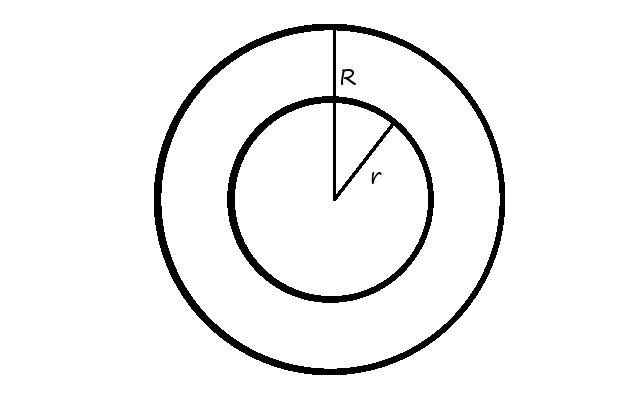
\includegraphics[scale=0.3]{Front.png}
\quad
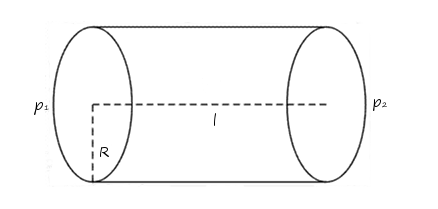
\includegraphics[scale=0.6]{Side.png}
\end{figure}
\\\\
A csődarab hossza $l$, és $p_1$, $p_2$ mennyiségek a cső két végén mért nyomásértékek. A felvett $R$ sugarú hengeren belül vegyünk fel $r<R$ sugarú hengert is. A feszültségtenzornak erre a hengerfelületre vett integrálja 0, ami  a \textit{Gauss-tétellel} is belátható:
$$
\oint\hat{\sigma}\;d\vec{A}=\int div(\hat{\sigma})dV=0
$$
Továbbá a hengerpaláston jelentkező nyírófeszültség csak vízszintes irányú, mivel az áramlás is vízszintes, tehát:
$$
\tau=\eta\;\frac{dv_x}{dr}
$$
A fedőlapokon a nyomásból is adódhat erő.
Az eddigiek alapján felírható a nyíróerők egyenlete:
\begin{equation}
F=A\;\eta\;\frac{dv_x}{dr},
\end{equation}
ahol $A=2r\pi l$ a hengerpalást felszíne.\\\\
A munkatétel pedig a következő módon írható fel:
\begin{equation}
\bigg(\oint\hat{\sigma}\;d\vec{A}\bigg)_x=2r\pi l\eta\;\frac{dv_x}{dr}\;+\;p_1r^2\pi\;-\;p_2r^2\pi=0
\end{equation}
Ezt az egynletet átalakítva és leegyszerűsítve a következő egyszerű alakra vezethetjük vissza a problémát:$$
\frac{dv_x}{dr}=\frac{p_2-p_1}{2l\eta}r,
$$
és ennek a megoldása:
\begin{equation}
v_x(r)=-\frac{p_1-p_2}{4l\eta}r^2+c
\end{equation}
A határfeltétlekből határozható meg az integrációs konstans. Feltehetjük, hogy a cső belső felülete miatt az áramlás sebessége a felszínen ($v_x(R)$) 0:
\begin{equation}
v_x(r)=\frac{p_1-p_2}{4l\eta}(R^2-r^2)
\end{equation}
Ebből az összefüggésből látszik, hogy a csőben egy parabolikus sebességprofil alakul ki.
\subsection*{Az átáramlott anyag mennyisége}
Tovább vizsgálható a probléma, ha felírjuk a kontinuitási egyenletet:
\begin{equation}
\frac{\partial \rho}{\partial t}\;+\;div(\rho\vec{v})=0,
\end{equation}
ami az anyagmegmaradást is kimondja. Tehát időegység alatt a cső keresztmetszetén átfolyó anyag mennyisége állandó. Az egységnyi idő alatt átfolyó anyag mennyiségét jelölje $\dot{\Phi}$, és ezek alapján az alábbi összefüggés teljesül (ahol integráláskor úgy daraboljuk fel az adott köralakú keresztemetszetet, hogy végül koncentrikus körgyűrűket kelljen összegeznünk):
\begin{equation}
\dot{\Phi}=\bigg(\int \rho \vec{v}\;d\vec{A}\bigg)_x=\int_{0}^{R} 2r\pi\;dr\; \frac{p_1-p_2}{4l\eta}(R^2-r^2)
\end{equation}
Az integrálást elvégezve a következő eredményt kapjuk:
\begin{equation}
\dot{\Phi}=\frac{\pi}{8}\;\frac{\rho}{l\eta}\;(p_1-p_2)R^4
\end{equation}
Ez az ún. \textit{Hagen-Poiseuille-összefüggés}. Itt az $R^4$ tényező az igazán érdekes, mivel ez azt jelenti, hogy kétszer akkora sugarú cső esetén az átáramlott anyag mennyisége 16-szorosára nő, és ez igen számottevő ugrás, amit számos alkalmazásban ki is használnak.
\subsection*{Kapcsolat a \textit{Bernoulli-törvénnyel}}
A \textit{Navier-Stokes-egyenlet} megfelelő tagjait elhagyva ilyen alakra hozható:
\begin{equation}
\rho(\vec{v}\,\vec{\nabla})\vec{v}\;=\;-grad(p)
\end{equation}
Ezek után felhasználhatjuk a következő azonosságot:
$$\vec{v}\times(rot(\vec{v}))=grad\bigg(\frac{|\vec{v}|^2}{2}\bigg)-(\vec{v}\,\vec{\nabla})\vec{v}$$
Ha az áramlást örvénymentesnek tekintjük, akkor $rot(\vec{v})=0$, tehát tovább alakítva az egyenletet:
$$\rho\;grad\bigg(\frac{|\vec{v}|^2}{2}\bigg)=-grad(p)$$
ha feltételezzük azt is, hogy állandó sűrűségű folyadékkal dolgozunk, akkor az egyenletben szereplő mennyiségek egy gradiens alá vihetők, és a következő fog összefüggés lesz igaz a rendszerre:
\begin{equation}
\frac{|\vec{v}|^2}{2}\;+\;\frac{p}{\rho}=const.
\end{equation}
Az eredményünk pedig maga a \textit{Bernoulli-törvény}, ami - amint látható - a megfelelő egyszerűsítésekkel és közelítésekkel levezethető az általánosan teljesülő \textit{Stokes-Navier-egyenletből}.
\subsection*{\textit{Reynolds-szám}}
Ha feltesszük, hogy ismert a $v$ sebesség, akkor összehasonlíthatjuk a \textit{Navier-Stokes-egyenlet} egyik oldalán lévő sebességgel arányos
$$\eta\Delta\vec{v}\quad\sim\quad\eta\frac{v}{l^2}$$
és a másik oldalán lévő sebesség négyzetével arányos
$$\rho(\vec{v}\,\vec{\nabla})\vec{v}\quad\sim\quad\rho\frac{v^2}{l}$$
tagokat a fenti becslések alapján a következő módon:
\begin{equation}
\frac{\rho\,\frac{v^2}{l}}{\eta\, \frac{v}{l^2}}=\frac{\rho}{\eta}\,v\,l=R,
\end{equation}
ahol $\frac{\rho}{\eta}=\nu$ kinematikai viszkozitás. $R$ pedig az ún. \textit{Reynolds-szám}, ami egy dimenzió nélküli arányszám, és lehet következtetni az értékéből arra, hogy az adott áramlás laminális vagy turbulens (a küszöb, ami felett turbulens az áramlás általában $R\approx1000$-nél van). A \textit{Reynolds-szám} jelentősége hasonlósági áramlásoknál érhető tetten igazán, mivel ha két probléma $R$-je megegyezik, akkor könnyen számolható egyik a másikból. 
\end{document}